\documentclass[a4paper,12pt]{article}
\usepackage{graphicx}
\usepackage[left=2.5cm, right=2.5cm, top=3cm, bottom=3cm]{geometry}
\usepackage{amsmath, amsthm, amssymb}
\usepackage[left=2.5cm, right=2.5cm, top=3cm, bottom=3cm]{geometry}
\usepackage[hidelinks]{hyperref}
\usepackage[spanish]{babel}
\usepackage{cite}
\usepackage{color}
\usepackage{url}

\bibliographystyle{plain}
\begin{document}
    \title{\huge \textbf{MOOGLE!}}
    \author{Diego Manuel Viera Martínez}
    \date{julio , 2023}
    \maketitle
    \begin{center}
        
\includegraphics[scale=0.7]{Pictures/matcom.jpg}
        \label{fig:logo}
    \end{center}
    \begin{center}
        \large Primer proyecto de programación
    \end{center}
    \newpage 
    \section{Funcionalidades}\label{sec:Funcionalidades}
    \subsection{Buscador:}\label{sub:Buscador}
    -Busca hasta los 5 documentos más relevantes según su búsqueda y los
    ordena de mayor a menor relevancia, muestra el título y el snippet.
    Si no hay exactamente 5 o más de 5 documentos muestra solo los documentos 
    encontrados, si ningún documento es relevante, informa que no hay resultados para la búsqueda.

    \begin{center}
        \includegraphics[scale=0.3]{Pictures/EjBúsqueda.JPEG}
    \end{center}

    \subsection{Snippet:}\label{sub:Snippet}
    -El snippet representa una porción del texto
    en el cual se encuentra por primera vez la palabra de la búsqueda
    con mayor importancia para el documento.
    
    \begin{center}
        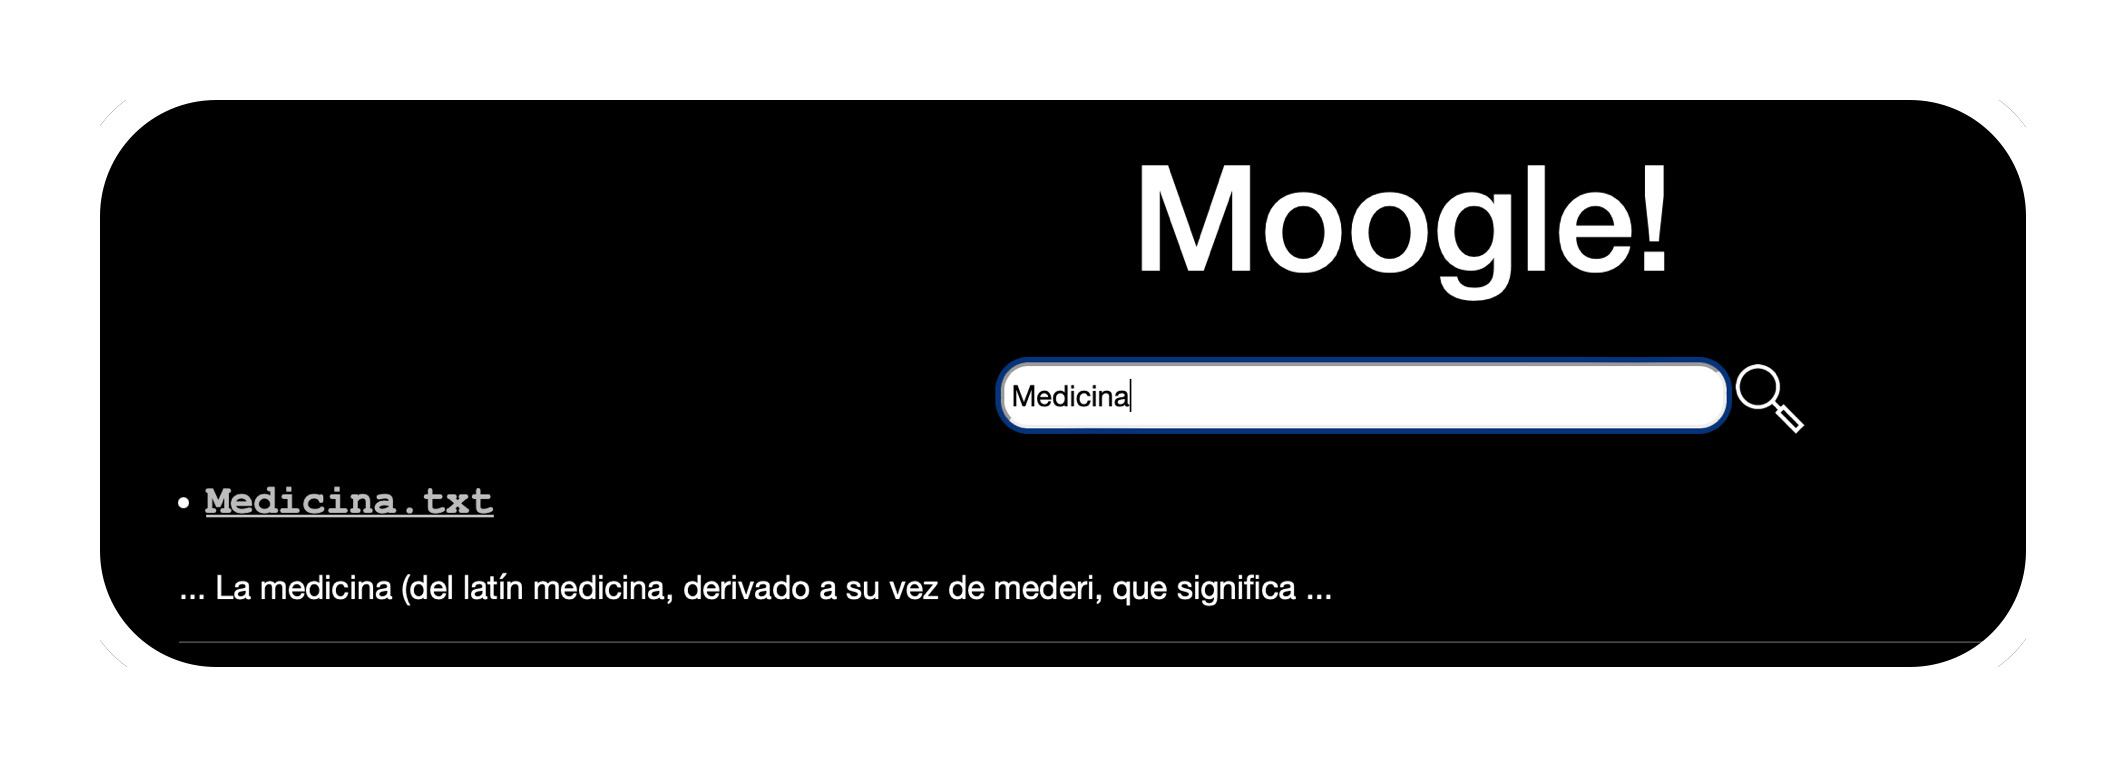
\includegraphics[scale=0.2]{Pictures/EjSnippet.JPEG}
    \end{center}

    \newpage

    \subsection{Suggestion}\label{sub:Suggestion}
    -Si la búsqueda contiene una palabra que no aparece en ninguno de
    los documentos, hace una sugerencia de una palabra corregida
    que si existe en la base de datos.
    \begin{center}
        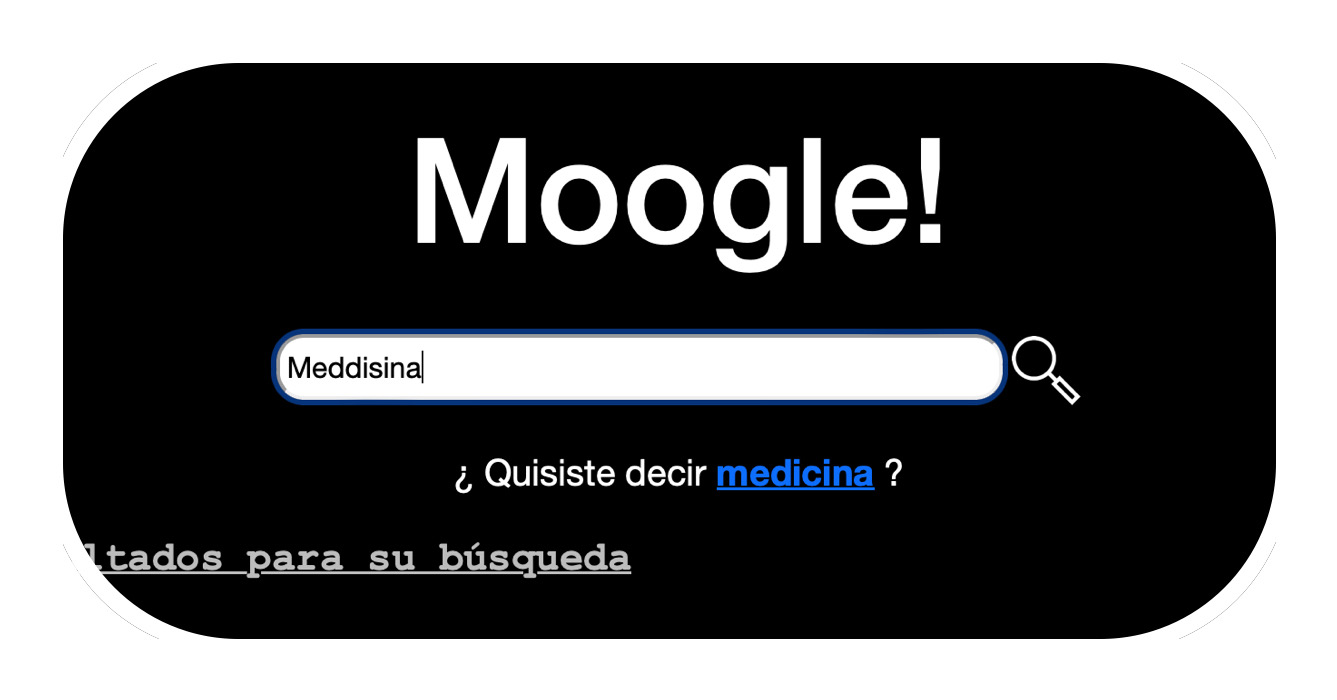
\includegraphics[scale=0.2]{Pictures/EjSuggestion.JPEG}
    \end{center}
    \subsubsection{Ejemplo}
    Escribe ramak (esta palabra no existe) y luego sugiere (rama), al tocar este hipervínculo
    hace una nueva búsqueda con la palabra sugerida.
    \subsection{Abrir Documentos}\label{sub:OpenDocs}
    -Al dar clic sobre el nombre de los txt , abre una nueva ventana mostrando el contenido del txt.
    \begin{center}
        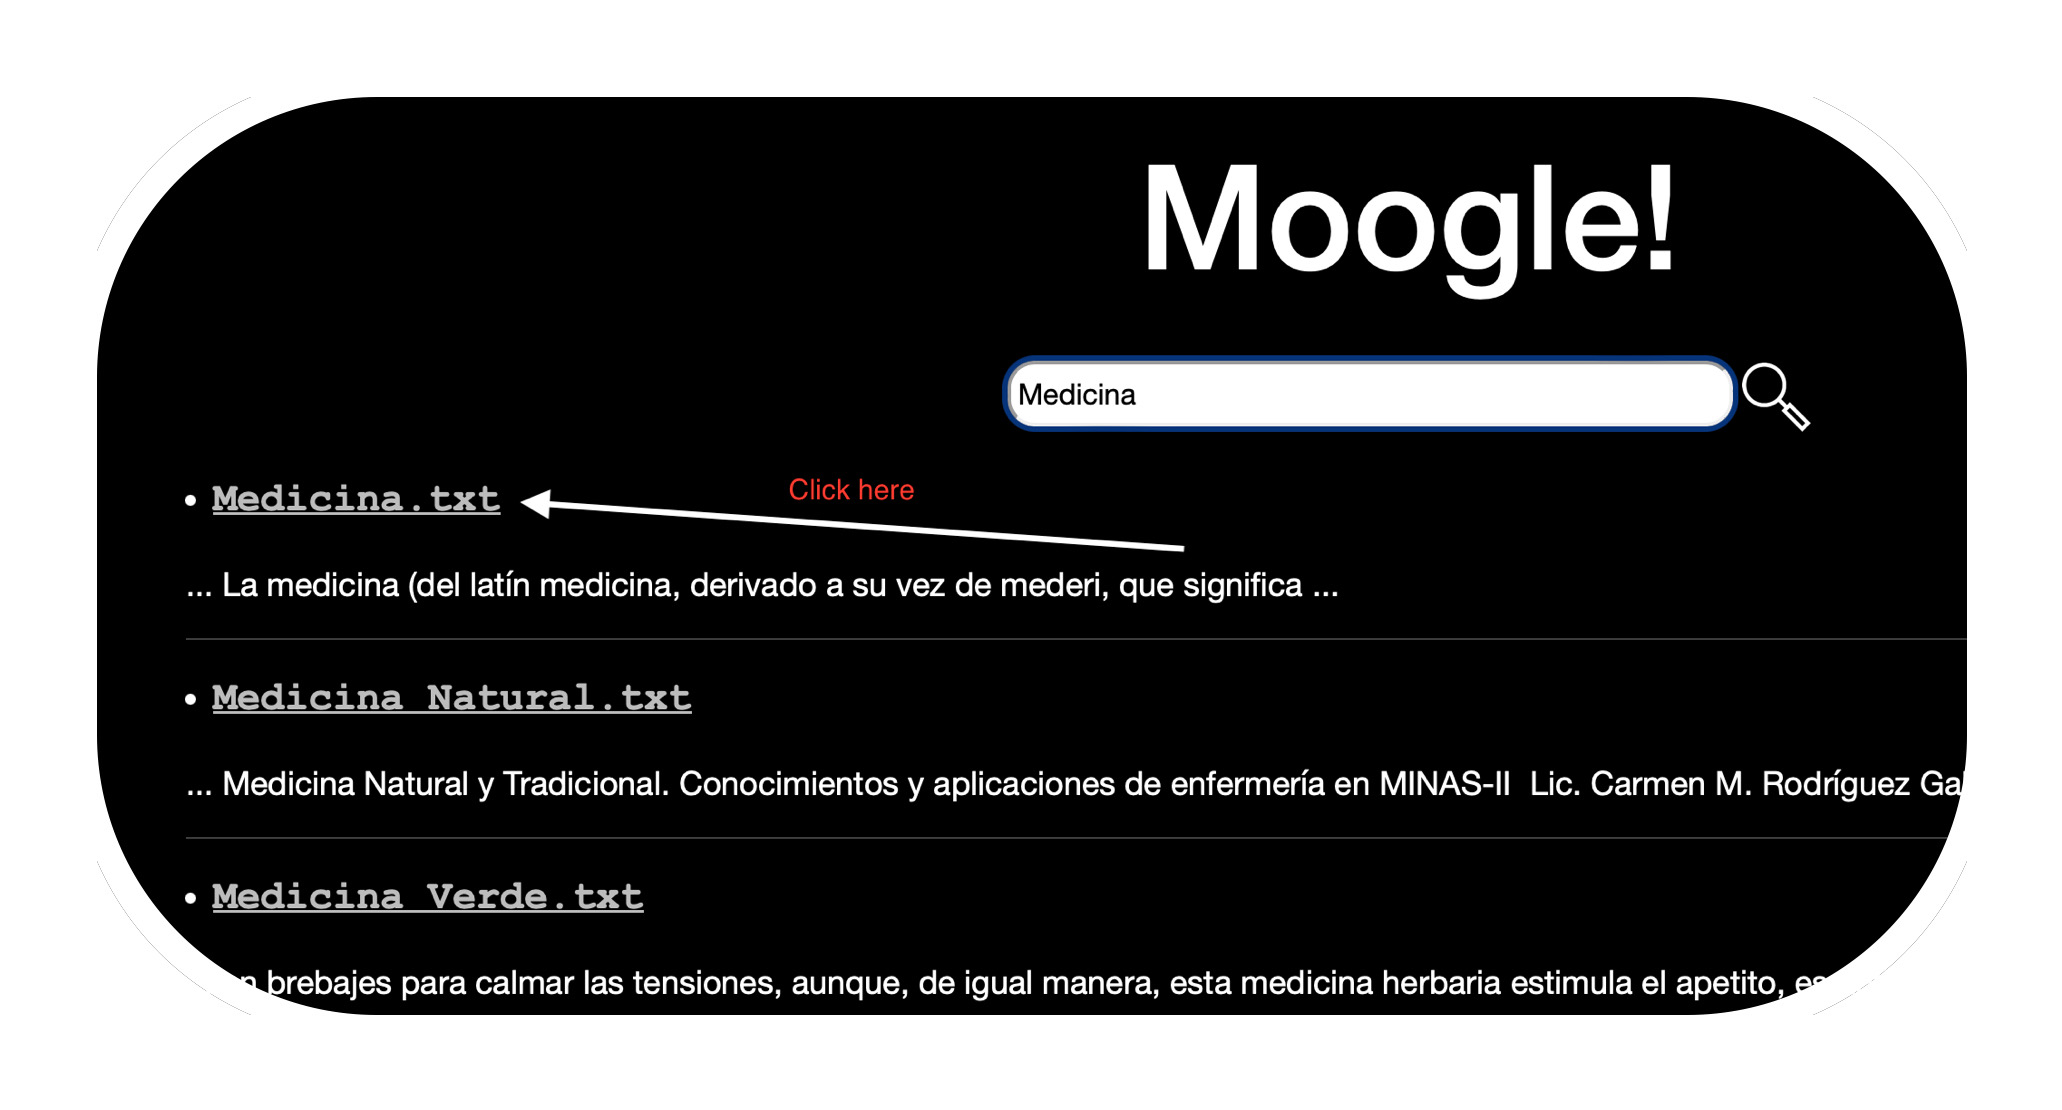
\includegraphics[scale=0.2]{Pictures/EjOpenDocs.JPEG}
    \end{center}

    \newpage

    \section{Explicación del código}\label{sec:explicacion}
    \subsection{Class Tools}\label{sub:Tools}
    -La clase Tools, primeramente obtiene las direcciones de cada documento y 
    las almacena (DireccionTextos), Almacena en (textos) los textos ya leídos como string,
    utilizo (FilesNames) para guardar solo los nombres de los textos,
    almacena en (Text-Words) las listas de palabras tokenizadas de cada
    documento(esto lo utilizo para obtener cuantas palabras tiene el documento).

    \subsubsection{Tools contiene el método de inicialización GetValues()}
    -Este método lee los textos y los almacena en (Tools.textos),
    le da los valores a: TFxIDF.TodasLasPalabras(Obtiene todas las palabras sin
    repetirse y almacena además en cuentos documentos aparece),
    TFxIDF.DiccionarioDeCadaDocumento (Crea un diccionario para cada documento que contiene las palabras de ese documento sin repetirse con el valor de cuantas veces aparece en el documento).
    Obtiene los nombres de los textos y los almacena en (Tools.FilesNames).
    \vspace{0.5cm}

    -Finalmente actualiza los valores de TFxIDF.DiccionarioDeCadaDocumento calculando el TF * IDF
    de cada palabra de cada diccionario , utilizando los valores de TFxIDF.DiccionarioDeCadaDocumento 
    (obtengo la cantidad de veces que se repite la palabra en el documento) y lo divido entre la cantidad
    de palabras del documento, obteniendo así el TF; con TFxIDF.Con TodasLasPalabras obtengo en cuantos documentos aparece la palabra , luego para
    calcular el IDF [log(cantidad de documentos / la cantidad de documentos donde aparece la palabra)].

    \begin{equation}\label{eq:TF}
        TF = \frac{Repeticiones\hspace{0.1cm}de\hspace{0.1cm} la\hspace{0.1cm} palabra\hspace{0.1cm} en\hspace{0.1cm} el\hspace{0.1cm} documento}{Cantidad\hspace{0.1cm} de\hspace{0.1cm} palabras\hspace{0.1cm} del\hspace{0.1cm} documento}
    \end{equation}
    \vspace{1cm}
    \begin{equation}
        IDF = \log{\frac{Cantidad \hspace{0.1cm}de\hspace{0.1cm} documentos}{Cantidad \hspace{0.1cm}de \hspace{0.1cm}documentos\hspace{0.1cm} que\hspace{0.1cm} contiene \hspace{0.1cm}la \hspace{0.1cm}palabra}}
    \end{equation}
    \vspace{1cm}
    \begin{equation}\label{eq:TF*IDF}
        TF-IDF = TF*IDF
    \end{equation}

    \vspace{1cm}

    -Esta clase contiene además el método Separar-palabras(string texto), 
    el cual retorna una lista de las palabras tokenizadas del texto
    (necesario para crear los diccionarios para cada documento).
    
    \newpage

    \subsection{Class TFxIDF}\label{sub:TFxIDF}

    -La clase TFxIDF tiene las siguientes propiedades:
    \vspace{1cm}

    - ( Dictionary<string , double> TodasLasPalabras ), 
    contiene todas las palabras de todos los documentos sin repetirse, almacenando a su vez , en cuántos documentos se encuentra cada palabra (necesario para calcular IDF).

    \vspace{1cm}

    - ( List < Dictionary < string , double > DiccionarioDeCadaDocumento ),
    contiene los diccionarios para cada documento por separado ( Cada elemento de la lista reperesenta el diccionario para el documento correspondiente ) los diccionarios almacenan las palabras del texto correspondiente sin repetirse , con el valor de la palabra calcualdo en el método de inicialización GetValues() de la clase Tools utilizando TF * IDF

    \vspace{1cm}
    2.2-TFxIDF contiene el método Calcular-Tf-Idf-query(string query) el cual devuelve un Dictionary<string , double> vectorquery , de las palabras del query sin repetirse con su valor (TF * IDF).

    \subsection{Class Similitud-Coseno}\label{sub:Similitud-Coseno}

    Contiene el método Calcular-Similitud-Coseno(Dictionary<string , double> vectorquery, Dictionary<string , double> Doc), en éste método se utiliza el calculo de similitud coseno[(Multiplicación escalar de los vectores) / (Multiplicación de los módulos de los vectores)], el cual expresa que tan parecidos son dos vectores
    (Expresamos nuestros textos como vectores). Nuestros vectores serían:
    (Dictionary<string , double> vectorquery) y (Dictionary<string , double> Doc). Calculando de esta forma el score de cada texto respecto al query.

    \vspace{1cm}

    -El método ScoreTop(string query) utiliza el método Calcular-Similitud-Coseno (Dictionary<string , double> vectorquery, Dictionary<string , double> Doc) para cada texto y devuelve una lista de los textos con score diferente de 0 , ordenados de mayor score a menor score

    \vspace{1cm}
    Fórmula de similitud coseno:
    \begin{equation}
        SC = \cos \theta = \frac{A * B}{\parallel A \parallel \parallel B \parallel} = \frac{\sum_{n = 1}^{n} A_i B_i  }{\sqrt{\sum_{n = 1}^{n} A^2_i} \sqrt{\sum_{n = 1}^{n} B^2_i} }
    \end{equation}

    \newpage

    \subsection{Proceso final}\label{sub:finalprocces}
    En el script Moogle.cs en el método Query llámo al método ScoreTop(string query) y obtengo mi lista de documentos más relevantes según el query, creo un array del tipo SearchItem (SearchItem[] item), añado hasta los 5 documentos más relevantes y finalmente retorno una instancia del tipo SearchResult(item , suggestion).

    \section{Opcionales}\label{sec:Opcionales}
    
    \subsection{Snippet}\label{sub:Explain Snippet}
    -Para el snippet primeramente busco con el método BestWord(Dictionary<string , double> vectorquery , int index) la palabra más relevante de mi query según el documento. Luego con el método snippet(string BestWord , int index-of-text) , busco el índice de la primera aparición de mi BestWord en el documento y creo un rango de hasta 140 caractéres a partir de este índice, creando de esta forma una porción del texto que contiene la palabra del query más relevante para el documento.

    \subsection{Suggestion}\label{sub:Explain Suggestion}
    -Para la sugerencia utilizo el algoritmo de Levenshtein, el cual expresa que tan parecidas son dos palabras, cree un método utilizando
    este algoritmo [LevenshteinDistance(string s , string t)], este retorna un int que representa la cantidad de cambios que deben realizarse para que las palabras sean iguales. Luego el método Suggestion(Dictionary<string , double> vectorquery)
    toma cada palabra de la búsqueda y verifica que existe en \\Tools.TodasLasPalabras, si esta existe mantiene la palabra tal como está y la añade a una lista resultante, si no existe la palabra utilizo el método de LevenshteinDistance(string s , string t)
    , para comparar mi palabra no existente con todas las palabras de Tools.TodasLasPalabras, y quedarme con la que menos cambios deben relaizarce (si varias palabras tienen la misma cantidad de cambios, me quedo simpre con la primera que encuentre con este mínimo de cambios)
    , la añado la palabra con el mínimo
    de cambios a mi lista resultante y luego creo un string a partir de esta lista , iterando por todas las palabras de query y corrigíendolas.

    \subsection{Abrir documentos}\label{sub:Explain OpenDocs}
    En el script index.razor cree un método OpenTxt(string title) donde utlizo la clase Process de System.Diagnostics.
    Luego en donde se muestra el título añadí un hipervínculo con un evento @onclick que llama al método OpenTxt(item.Title)

\end{document}